\subsubsection{Completed Main Matrix and Crossed F/G Robustness}

All 153 logical main F rows (17 contracts, three registered recipes and three F seeds) now have complete seven-view predictions and independent scores, including six input-binding replacements for the F0 controls. Local aggregation recomputed 122598 serialized confusion matrices and 70056 repair-minus-damage nets. ManyRx uses its registered ten classes; all other contracts use six. Source/date/TX contracts are kept separate. Native T1 and matched Sup/ordinary-PL differ in their registered training recipes, including augmentation and forward exposure, so their differences do not isolate a single component.

\begin{table*}[t]\centering\footnotesize\setlength{\tabcolsep}{4pt}

\caption{Complete native T1 main matrix: Accuracy in percent, mean$\pm$sample SD over three F seeds conditional on the fixed G-LU per contract. S6 averages the six scenes within seed. Different physical target sets are not pooled.}\label{tab:main153}

\begin{tabular}{lrrrrrr}\toprule Contract & Packets/view & Classes & Raw clean & Raw S6 & G-LU S6 & Paired G gain (points)\\\midrule

F0 & 168000 & 6 & $84.394\pm0.916$ & $70.601\pm1.062$ & $77.647\pm0.846$ & $7.046\pm0.595$\\

F1 & 168000 & 6 & $73.167\pm0.865$ & $61.602\pm0.714$ & $66.850\pm0.421$ & $5.248\pm0.865$\\

F2 & 168000 & 6 & $81.738\pm1.403$ & $71.945\pm0.536$ & $74.710\pm1.408$ & $2.764\pm0.914$\\

ManyRx & 123021 & 10 & $83.883\pm0.248$ & $63.523\pm0.472$ & $72.192\pm0.385$ & $8.669\pm0.136$\\

chrono & 168000 & 6 & $83.707\pm1.329$ & $70.491\pm0.934$ & $76.245\pm0.366$ & $5.755\pm0.594$\\

label01 & 168000 & 6 & $81.376\pm0.382$ & $69.919\pm0.054$ & $73.561\pm0.686$ & $3.642\pm0.660$\\

label05 & 168000 & 6 & $84.096\pm1.030$ & $70.552\pm0.439$ & $75.695\pm0.619$ & $5.143\pm0.608$\\

m1-natural & 144000 & 6 & $50.435\pm1.356$ & $48.355\pm1.388$ & $53.564\pm0.281$ & $5.209\pm1.193$\\

m2-natural & 144000 & 6 & $69.081\pm2.003$ & $58.793\pm0.769$ & $62.527\pm1.397$ & $3.734\pm0.765$\\

m3-natural & 144000 & 6 & $82.120\pm1.148$ & $69.835\pm0.593$ & $72.438\pm1.027$ & $2.604\pm0.682$\\

m4-natural & 144000 & 6 & $82.292\pm0.558$ & $68.690\pm0.562$ & $73.468\pm0.431$ & $4.778\pm0.956$\\

m6-natural & 144000 & 6 & $86.551\pm0.275$ & $72.872\pm0.399$ & $75.059\pm0.402$ & $2.187\pm0.474$\\

m1-fixed & 144000 & 6 & $49.087\pm0.834$ & $47.545\pm1.257$ & $50.401\pm0.823$ & $2.856\pm1.063$\\

m2-fixed & 144000 & 6 & $66.691\pm1.659$ & $58.648\pm1.107$ & $61.602\pm1.008$ & $2.954\pm0.958$\\

m3-fixed & 144000 & 6 & $79.422\pm1.728$ & $68.631\pm0.787$ & $69.616\pm0.578$ & $0.985\pm0.542$\\

m4-fixed & 144000 & 6 & $80.141\pm0.557$ & $68.054\pm0.499$ & $72.181\pm0.312$ & $4.126\pm0.269$\\

m6-fixed & 144000 & 6 & $83.735\pm0.537$ & $71.827\pm0.646$ & $74.203\pm0.267$ & $2.377\pm0.897$\\

\bottomrule\end{tabular}\end{table*}

All 17 native-T1 six-scene G-LU/raw mean gains are positive, ranging from 0.9852 to 8.6694 points, but five contracts have nonpositive clean mean differences. The largest clean reduction is the one-source fixed-budget condition ($-0.6044\pm0.2159$ points). Native T1 minus the supervised and ordinary-PL controls under G-LU is nonpositive in three and five of the 17 six-scene conditions, respectively. These negative and nonmonotonic outcomes are retained; target results do not change the fixed default or queue.

\begin{figure*}[t]\centering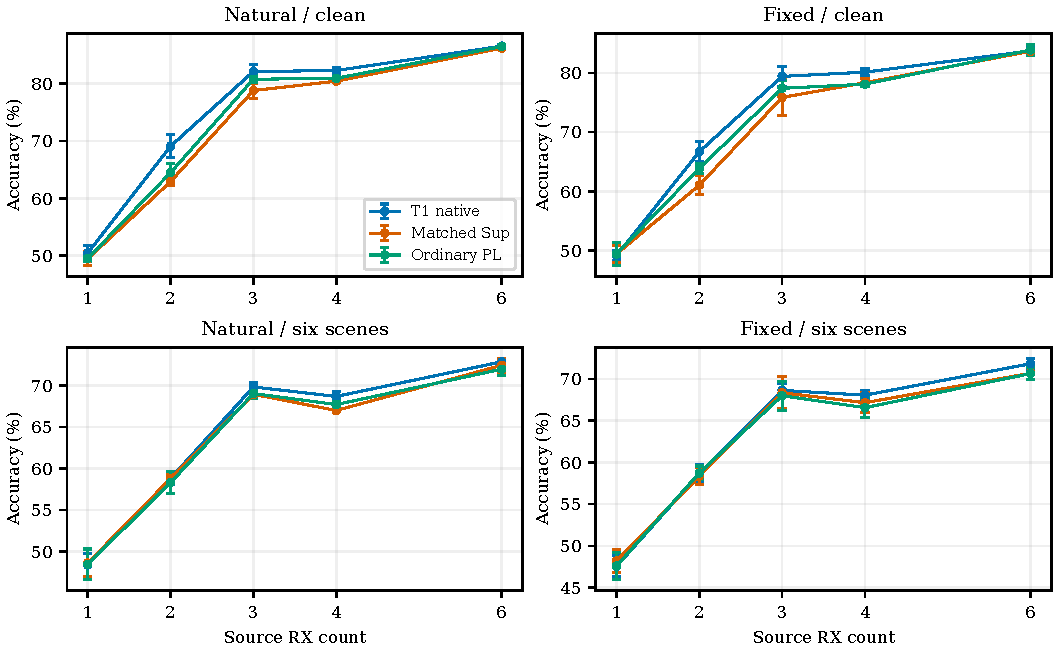
\includegraphics[width=\textwidth]{images/main153/main_sourcecount_raw.pdf}\caption{Matched PAMF source-count curves on raw inputs, three F seeds. The same six target RX/144000 packets are used at every point; no m=5 point or seven-target F0 result is inserted. Error bars are sample SD.}\label{fig:main-source-raw}\end{figure*}

\begin{figure*}[t]\centering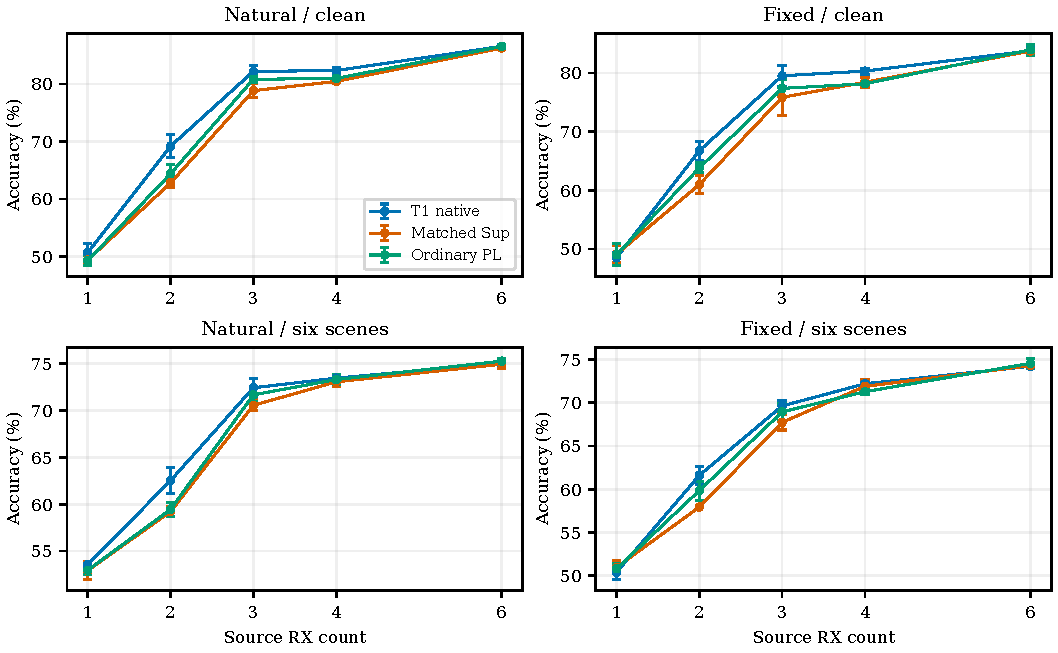
\includegraphics[width=\textwidth]{images/main153/main_sourcecount_DURA_LU.pdf}\caption{The same trained F models after exact-contract frozen DURA-LU. These curves use U through G even for the supervised F.}\label{fig:main-source-g}\end{figure*}

\begin{figure*}[t]\centering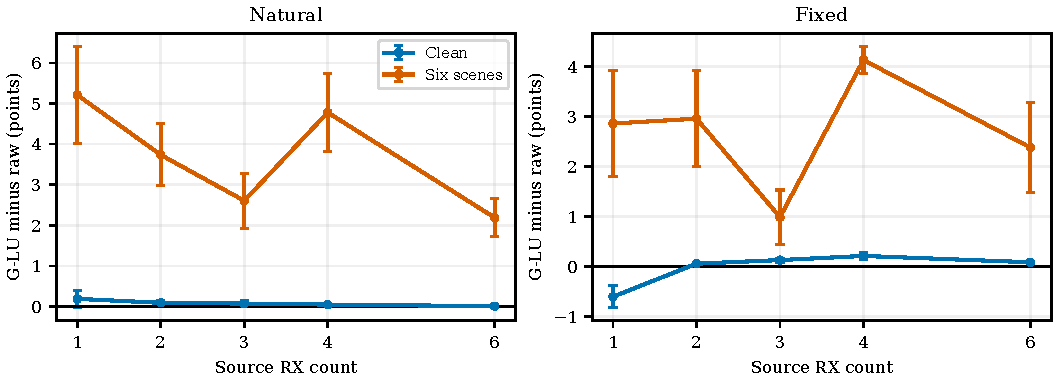
\includegraphics[width=\textwidth]{images/main153/main_restoration_gain.pdf}\caption{Within-F-seed G-LU/raw paired gains, preserving all clean reductions and nonmonotonic source-count effects.}\label{fig:main-gain}\end{figure*}

The predeclared m3-natural robustness panel is also complete: two extra G seeds add six readouts to the original fixed-G column, yielding the complete three-F by three-G grid (Fig.~\ref{fig:main-crossed}). Same-F raw confusion matrices are identical across G choices. Each fixed-G column describes F variability; the three diagonal joint F/G seeds are three complete-system training-seed repetitions. The nine crossed cells are not nine independent complete-system repetitions.

\begin{table}[t]\centering\footnotesize\caption{m3-natural crossed robustness (Accuracy,\%).}\label{tab:main-crossed}\begin{tabular}{lrr}\toprule Condition & Clean & S6\\\midrule

Fixed G01 & $82.191\pm1.082$ & $72.438\pm1.027$\\

Fixed G02 & $82.090\pm1.225$ & $72.788\pm1.015$\\

Fixed G03 & $82.118\pm1.184$ & $72.849\pm1.210$\\

Joint diagonal & $82.100\pm1.219$ & $72.822\pm1.037$\\

\bottomrule\end{tabular}\end{table}

\begin{figure}[t]\centering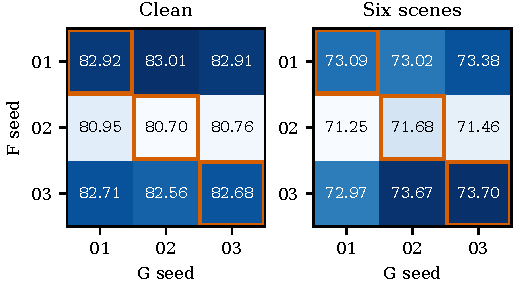
\includegraphics[width=\columnwidth]{images/main153/main_m3_crossed.pdf}\caption{Complete m3-natural F/G seed grid. Red boxes identify diagonal joint-seed repetitions; all cells are reported.}\label{fig:main-crossed}\end{figure}

The 150 newly trained main F models sum to 245.675 shared-worker elapsed hours; all 153 logical sources including reused historical T1 segments sum to 250.292 hours. The 35 new complete G lineages contain 280 fixed E20 stages (5600 model-epochs/1383200 updates), summing to 181.730 shared-worker elapsed hours, including the two additional crossed G seeds. These are cumulative costs under shared contention, not exclusive GPU hours or wall-clock speedup measurements. Original fixed-F0 G ancestry, shared observation/IQ-cache production, the 21 G students and prediction cost remain separate. Per-scene/RX/TX/day Accuracy, Macro-F1, chrono auxiliary tasks, net corrections and every cost record are preserved for reproduction. The PL-F/G-L supplement and external-method DURA readouts remain separate pending panels.
